\chapter{Data Formats}
\label{sec:DataFormats}

Rather than creating a new format, or trying to describe the same structure in each different document format, a single common highly portable standard was chosen.

JSON\cite{JSON}, designed to be used as a plain-text data interchange format for the web has been ported to a vast set of languages, 

\section{Data Structure}
By using JSONs \textit{object} data type, we can indefinitely nest fields within fields.
It is this feature that allows us to build tree structures using JSON, and build up complex relationships between parent and child fields.

This specification makes extensive use of this mechanism to provide conflict-less field-name spaces in to which tools and libraries can have relatively free rein to define their own structures.

\begin{figure}[ht!]
    \centering
    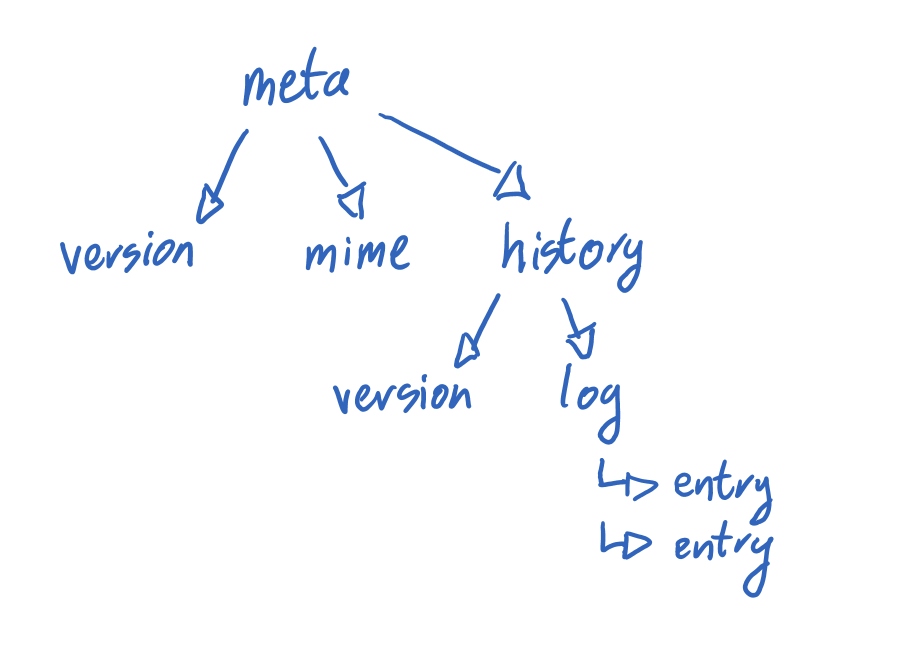
\includegraphics[width=0.5\textwidth]{diagrams/meta-tree.png}
    \caption{An example of the tree-structure JSON affords the metaheader specification}
    \label{structure:meta-tree}
\end{figure}

\section{Semantic Versioning}
\label{sec:SemanticVersioning}
Semantic version fields, denoted by the \texttt{\_\_version\_\_} field name use string format values, but must strictly follow the Semantic Versioning (SemVer) scheme of \texttt{major.minor.patch}, as a dotted-triple\footnote{`Dotted-Triple' - A sequence of three independent sub items separated by a dot, usually numeric, but not required to be, and if numeric, multiple number bases can be used in separated sections.} as defined in the latest draft of the specification.

The three sections of the semantic version field are (currently, at the time of writing according to semver 2.0.0) defined as follows:
\begin{enumerate}
    \item[major] Version when you make incompatible API changes,
    \item[minor] Version when you add functionality in a backwards-compatible manner, and
    \item[patch] Version when you make backwards-compatible bug fixes.
\end{enumerate}

It should be noted that the \texttt{minor} and \texttt{patch} fields must only increment if the changes made are backward-compatible with the previous versions. 
If they are not, then the \texttt{major} version should tick over and reset the other two to indicate the break in compatibility.

The current draft format for semantic versioning can be found at \url{http://semver.org/}